\documentclass[12pt, a4paper]{article}
\usepackage{fontspec}
\setmainfont{Times New Roman}
\usepackage[UTF8]{ctex}
\usepackage{listings}
\usepackage{array}
\usepackage{geometry}
\geometry{a4paper, scale=0.75}
\usepackage{ctex}
\usepackage{amsmath}
\usepackage{epsfig}
\usepackage{graphicx}
\usepackage{epstopdf}
\usepackage{cite}
\usepackage{indentfirst}
\setlength{\parindent}{2em}
\setlength\parskip{.3 \baselineskip}
\usepackage{graphicx}
\usepackage{float}
\usepackage{subfigure}

\begin{document}
	\begin{center}
		\vspace{0.2in}
		\noindent{\fontsize{20pt}{1em}\selectfont\textbf{通信电路\quad 第八周作业}} \\ [12pt]
		\noindent{\fontsize{20pt}{1em}\textbf{Cadence报告}}  \\ [12pt]
		{\fontsize{14pt}{1.2em}\selectfont
			刘开济\\ [10pt]
			2019010973 \\ [10pt]
		}
	\end{center}
    \section{无源多相滤波器的仿真分析}
     无源多相滤波器原理图如下:
    \begin{figure}[H]
    	\centering
    	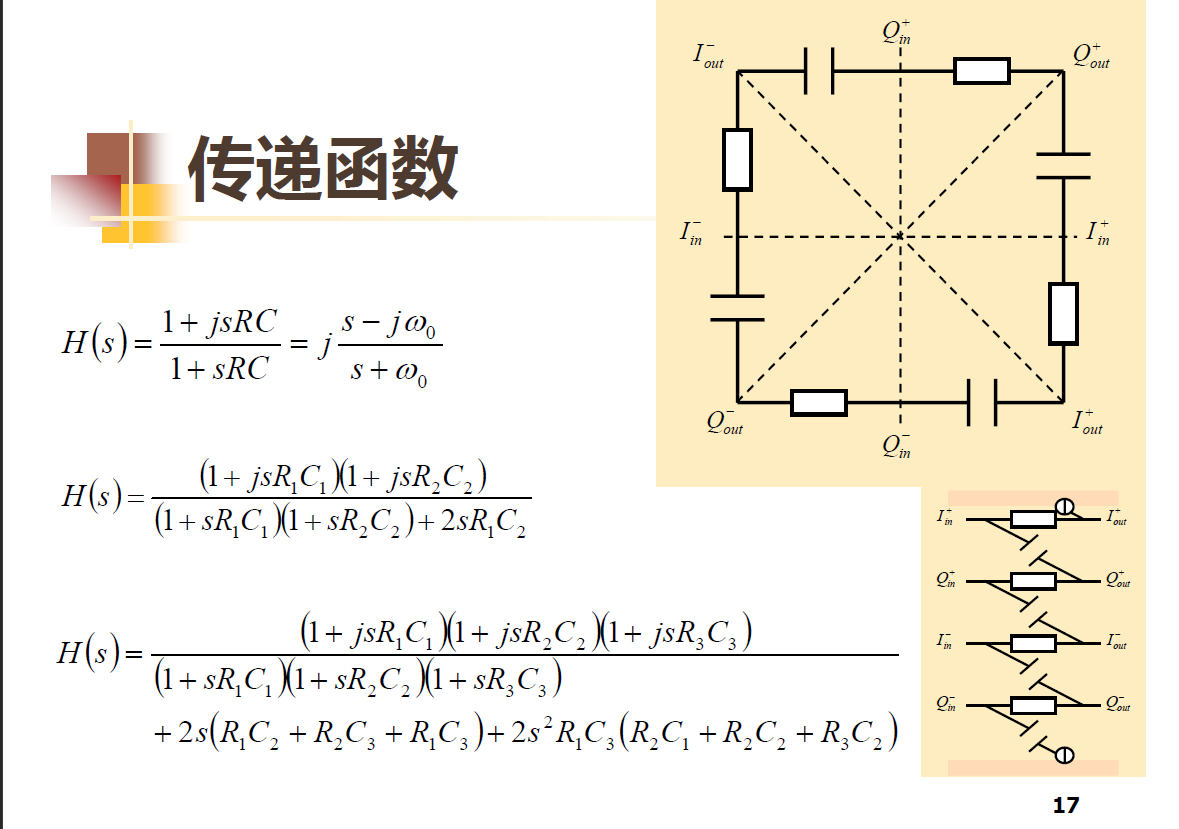
\includegraphics[width = 0.8\textwidth]{theory}
    	\caption{一阶无源多相滤波器电路拓扑}
    \end{figure}\par
    在无源多相滤波器中,电流只能从$I_{in}, Q_{in}$端口流入/流出,不能从$I_{out}, Q_{out}$端口流入/流出,故而有理论分析如下:
    \begin{gather}
    	Q_{out}^{+} = I_{in}^+ + \frac{Q_{in}^+ - I_{in}^+}{1 + sRC}\\
    	Q_{out}^{-} = I_{in}^- + \frac{Q_{in}^- - I_{in}^-}{1 + sRC}\\
    	I_{out}^{+} = Q_{in}^- + \frac{I_{in}^+ - Q_{in}^-}{1 + sRC}\\
    	I_{out}^{-} = Q_{in}^+ + \frac{I_{in}^- - Q_{in}^+}{1 + sRC}\\
    \end{gather}\par
    于是可得:
    \begin{equation}
    	H(s) = \frac{(I_{out}^+ - I_{out}^- ) + j(Q_{out}^+ - Q_{out}^-)}{(I_{in}^+ - I_{in}^- ) + j(Q_{in}^+ - Q_{in}^-)} = \frac{1 + jsRC}{1 + sRC} = j \frac{s - j\omega_0}{s + \omega_0)}
    \end{equation}\par
    考察其电路仿真如下:
     \begin{figure}[H]
    	\centering
    	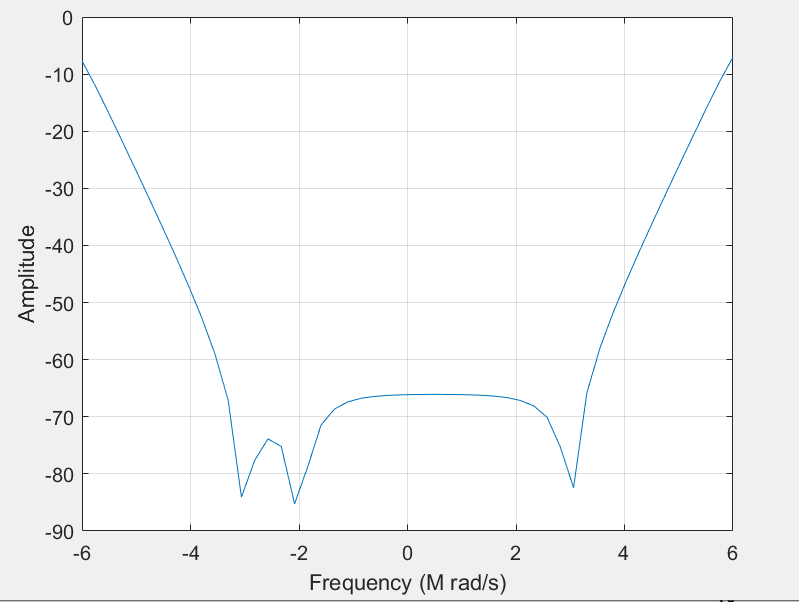
\includegraphics[width = 0.8\textwidth]{mag}
    	\caption{无源多相滤波器幅频特性数值例}
    \end{figure}\par
    扫描发现,$R_1$越大,$R_2$越小,则其-60dB带宽越大。
\end{document}